\documentclass{article}
\usepackage[english]{babel}
\usepackage{amsthm}
\usepackage{amsfonts} 
\usepackage[a4paper, margin=1in]{geometry} 
\usepackage{algorithm}
\usepackage{algorithmicx}
\usepackage{algpseudocode}
\usepackage{amsmath}
\usepackage{pgfplots}
\usepackage{graphicx}
\usepackage{caption}
\usepackage{subcaption}

\newtheorem*{remark}{Remark}
\setlength{\parindent}{0pt}
\hyphenpenalty=1000
\tolerance=1000
\sloppy



\begin{document}

\section*{Skupina 18: Kemijski grafi}
\textit{Avtorja: David Planinšek Šilc, Lenart Žerdin \\ Datum: 20. 12. 2024 \\}

\subsection*{Opis problema}
Najina naloga temelji na raziskovanju kemijskih grafov in njihovem
$\sigma_t^{f(n)}(G)$ indeksu. Zanima naju, kako se indeks v odvisnosti od
različnih $f(n)$ spreminja in katera stopenjska zaporedja grafa pridelajo njegov 
maksimum. Omejila sva se na funkcije $f(n) = \frac{1}{n}$ in $f(n) = c$ za 
$c \in (0, 1)$, kjer sva podrobneje gledala tiste $c$, ki so blizu $0$ in $1$.

\subsection*{Definicije}

\begin{enumerate}
    \item Graf je kemijski, če je neusmerjen, povezan in so vsa njegova vozlišča stopnje največ 4.
        Če ima kemijski graf $a_i$ vozlišč stopnje $i$, $1 \leq i \leq 4$,
        potem njegovo stopenjsko zaporedje označimo kot $(1^{a_1}, 2^{a_2}, 3^{a_3}, 4^{a_4})$. 

    \item Definiramo totalni $\sigma$-indeks iregularnosti, v angleščini
        `Total $\sigma$-irregularity', $\sigma_t^{f(n)}(G)$ kot:
        \[
        \sigma_t^{f(n)}(G) = \sum_{\{u,v\} \subseteq V(G)} \left| d_G(u) - d_G(v) \right|^{f(n)},
        \]
        kjer je $n = |V(G)|$ in je $f(n)$ funkcija, definirana za $n \geq 4$. 
\end{enumerate}

\subsection*{Izrek}
Naj bo $n \geq 7$, $f(n) \leq \log_3 \left( \frac{3n^2}{3n^2 - 8} \right)$, in naj bo $(1^{a_1}, 2^{a_2}, 3^{a_3}, 4^{a_4})$ stopenjsko zaporedje kemijskega grafa $G$ z maksimalno vrednostjo $\sigma_t^{f(n)}(G)$. Potem velja:
\begin{enumerate}
    \item Če $n = 4k - 1$, potem $a_1 = a_3 = a_4 = k$ in $a_2 = k - 1$.
    \item Če $n = 4k$, potem $a_1 = a_2 = a_3 = a_4 = k$.
    \item Če $n = 4k + 1$, potem $a_1 = a_2 = a_3 = k$ in $a_4 = k + 1$.
    \item Če $n = 4k + 2$, potem velja bodisi $a_1 = a_3 = k$ in $a_2 = a_4 = k + 1$, bodisi $a_1 = a_3 = k + 1$ in $a_2 = a_4 = k$. 
\end{enumerate}

Ker je za kemijske grafe razlika med stopnjami vozlišč omejena, domnevamo naslednje: 

\begin{itemize}
    \item \textbf{Domneva 1:} Isti grafi, kot v Izreku, imajo maksimalno vrednost za $\sigma_t^{f(n)}$, če je $f(n) = \frac{1}{n}$. 
    \item \textbf{Domneva 2:} Isti grafi, kot v Izreku, imajo maksimalno vrednost za $\sigma_t^{f(n)}$, če je $f(n) = c$, kjer je $c$ konstanta v intervalu $(0, 1)$. 

\end{itemize}

\subsection*{Algoritmi in psevdokode}
Za preverjanje domnev sva napisala algoritme, ki generirajo kemijske grafe in izračunajo njihov $\sigma_t^{f(n)}$ indeks.
Najprej sva se lotila sistematičnega iskanja za grafe z $n$ vozlišči, kjer je $n \in [7, 14]$, $n \in \mathbb{N}$.
Za večje grafe sva zaradi predolgega trajanja iskanja uporabila algoritma Hill climbing in Simulated annealing. Natančneje
za grafe velikosti $n \in [15, 20] \cup [50, 53] \cup [100, 103]$.

\subsubsection*{Sistematično iskanje}
Pri sistematičnem iskanju sva generirala vsa možna stopenjska zaporedja z uporabu knjižnice $nauty\_geng$, 
za različne $n$ in izračunala $\sigma_t^{f(n)}(G)$ za različne $f(n)$. Nato sva
izbrala tiste grafe, kjer je bila pri določenih $f(n)$ vrednostjo $\sigma_t^{f(n)}(G)$
največja.


\subsubsection*{Psevdokoda za sistematično iskanje}

\begin{algorithmic}[1]


\Function{GenerateUniqueChemicalGraphsConfigs}{$n$}
    \State $unique\_configs \gets []$
    \ForAll{$g$ v $graphs.nauty\_geng(f"{n} -c -D4")$}
        \State $config \gets DegreeConfiguration(g)$
        \If{$config \notin unique\_configs$}
            \State Dodaj $config$ v $unique\_configs$
        \EndIf
    \EndFor
    \State \Return $unique\_configs$
\EndFunction

\Function{SigmaTotalIrregularityFromConfig}{$config, f_n$}
    \ForAll{$config$ v $degree\_list$}
        \State compute $\sigma_t^{f(n)}(G)$
    \EndFor
    \State \Return $(config | \max(\sigma_t^{f(n)}(G)))$
\EndFunction
\end{algorithmic}

\vspace*{1cm}

\subsubsection*{Hill climbing algoritem}
Hill climbing algoritem je optimizacijski algoritem,
ki iterativno izboljšuje trenutno rešitev tako, da na vsakem koraku
poišče sosednjo rešitev z boljšo, v najinem primeru večjo, $\sigma_t^{f(n)}(G)$
vrednostjo. Algoritem sva ustavila po 100000 iteracijah. 

\subsubsection*{Psevdokoda za Hill climbing algoritem}



    \begin{algorithmic}[1]
    
    \Function{GenerateInitialGraph}{$n$}
        \State Ustvarimo drevo na n vozliščih
    \EndFunction
    
    \Function{MutateGraph}{$g, u, v$}
        \If{$g$ vsebuje povezavo $(u, v)$}
            \State Odstrani povezavo $(u, v)$ iz $g$
            \If{$g$ je povezan}
                \State \Return $g$
            \Else
                \State Dodaj nazaj $(u, v)$
                \State \Return $g$
            \EndIf
        \Else
            \State Dodaj povezavo $(u, v)$ v $g$
            \If{$\max(\text{degree}(g)) \leq 4$}
                \State \Return $g$
            \Else
                \State Odstrani $(u, v)$
                \State \Return $g$ 
            \EndIf
        \EndIf
    \EndFunction 
    
    \end{algorithmic}

    \vspace*{1cm}
   
    \begin{algorithmic}[1]
    
    \Function{HillClimbing}{$n, f, iterations$}
        \State $current\_graph \gets$ GenerateInitialGraph($n$)
        \State $degree\_counts \gets$ seznam stopenj v $current\_graph$
    
        \For{$i$ in  range($iterations$)}
            \State $vertices \gets$ seznam vozlišč v $current\_graph$
            \State $(u, v) \gets$ naključno izbran par vozlišč iz $vertices$
            
            \State $original\_contribution \gets 0$
            \ForAll{$w$ v $vertices$}
                \If{$w \neq u$}
                    \State $org\_contribution += |degree\_counts[u] - degree\_counts[w]|^{f_n}$
                \EndIf
                \If{$w \neq v$ in $w \neq u$}
                    \State $org\_contribution += |degree\_counts[v] - degree\_counts[w]|^{f_n}$
                \EndIf
            \EndFor
    
            \State $new\_graph \gets$ MutateGraph($current\_graph, u, v$)
            \State $new\_degree\_counts \gets$ seznam stopenj v $new\_graph$
    
            \State $new\_contribution \gets 0$
            \ForAll{$w$ v $vertices$}
                \If{$w \neq u$}
                    \State $new\_contribution += |degre\_counts[u] - degree\_counts[w]|^{f_n}$
                \EndIf
                \If{$w \neq v$ in $w \neq u$}
                    \State $new\_contribution += |degree\_counts[v] - degree\_counts[w]|^{f_n}$
                \EndIf
            \EndFor
    
            \If{$new\_contribution > original\_contribution$}
                \State $current\_graph \gets new\_graph$
                \State $degree\_counts \gets new\_degree\_counts$
            \EndIf
        \EndFor
    
        \State $\sigma_t^{f(n)}(G) \gets 0$
        \ForAll{$(x, y) \in$ pari vozlišč v $current\_graph$}
            \State $\sigma_t^{f(n)}(G) += |degree(x) - degree(y)|^{f_n}$
        \EndFor
    
        \State \Return $(current\_graph, \sigma_t^{f(n)}(G))$
    \EndFunction 
    
    \end{algorithmic}
    

\subsubsection*{Simulated annealing algoritem}
Problem pri Hill climbing algoritmu je, da se lahko zatakne v lokalnem 
maksimumu. Simulated annealing algoritem je pristop, ki se temu izogne,
tako da včasih sprejema tudi slabše rešitve. Algoritem sva ustavila po
100000 iteracijah.

\subsubsection*{Psevdokoda za Simulated annealing algoritem}
    \begin{algorithmic}[1]
    \Function{Simulated Annealing}{$n,f_n,iterations, T, \alpha$}    
        \State $T= 1$
        \State $\alpha = 0.99$
        \State $\Delta \gets new\_contribution - original\_contribution$
        \If{$\Delta > 0$ \textbf{or} $random() < \exp(\Delta / T)$}
            \State $current\_graph \gets new\_graph$
            \State $degree\_counts \gets new\_degree\_counts$
        \EndIf
            
        \State $T \gets T \cdot \alpha$ 
    \EndFunction
    \end{algorithmic}


\vspace*{0.5cm}

\subsection*{Tabele in grafi}

\subsubsection*{Tabela za sistematično iskanje}

{\footnotesize
\[
\begin{array}{c|c|c|c|c|c|c|c|c|c|c}
    n & \frac{1}{n} & 0.0001 & 0.1  & 0.2 & 0.45 & 0.55 & 0.8 & 0.9 & 0.9995 \\
    \hline
    7  & (2, 1, 2, 2) & (2, 2, 2, 1) & (2, 1, 2, 2) & (2, 1, 2, 2) & (2, 1, 2, 2) & (3, 1, 1, 2) & (3, 0, 1, 3) & (3, 0, 1, 3) & (3, 0, 1, 3) &  \\
    8  & (2, 2, 2, 2) & (2, 2, 2, 2) & (2, 2, 2, 2) & (2, 2, 2, 2) & (3, 1, 1, 3) & (3, 1, 1, 3) & (3, 1, 1, 3) & (4, 0, 0, 4) & (4, 0, 0, 4) &  \\
    9  & (2, 2, 2, 3) & (2, 3, 2, 2) & (2, 2, 2, 3) & (2, 2, 2, 3) & (3, 2, 1, 3) & (3, 2, 1, 3) & (4, 1, 0, 4) & (4, 1, 0, 4) & (4, 1, 0, 4) &  \\
    10 & (3, 2, 3, 2) & (3, 2, 3, 2) & (3, 2, 3, 2) & (3, 2, 3, 2) & (4, 1, 2, 3) & (4, 1, 2, 3) & (5, 0, 1, 4) & (5, 0, 1, 4) & (5, 0, 1, 4) &  \\
    11 & (3, 2, 3, 3) & (3, 3, 3, 2) & (3, 2, 3, 3) & (3, 2, 3, 3) & (4, 2, 2, 3) & (4, 1, 2, 4) & (5, 0, 1, 5) & (5, 0, 1, 5) & (5, 0, 1, 5) &  \\
    12 & (3, 3, 3, 3) & (3, 3, 3, 3) & (3, 3, 3, 3) & (3, 3, 3, 3) & (4, 2, 2, 4) & (4, 2, 2, 4) & (5, 1, 1, 5) & (5, 1, 1, 5) & (6, 0, 0, 6) &  \\
    13 & (3, 3, 3, 4) & (3, 3, 3, 4) & (3, 3, 3, 4) & (3, 3, 3, 4) & (4, 3, 2, 4) & (4, 2, 2, 5) & (5, 1, 1, 6) & (6, 1, 0, 6) & (6, 1, 0, 6) &  \\
    14 & (4, 3, 4, 3) & (4, 3, 4, 3) & (4, 3, 4, 3) & (4, 3, 4, 3) & (5, 2, 3, 4) & (5, 2, 3, 4) & (6, 1, 2, 5) & (7, 0, 1, 6) & (7, 0, 1, 6) &  
\end{array}
\]
}

\vspace*{0.5cm}

\subsubsection*{Tabela za Hill climbing algoritem}

{\footnotesize
\[
\begin{array}{c|c|c|c|c|c|c|c|}
    n & \frac{1}{n} & 0.001 & 0.1 & 0.5 & 0.9 & 0.995 \\
    \hline
    15 & (4, 3, 4, 4) & (4, 3, 4, 4) & (5, 2, 3, 5) & (5, 2, 3, 5) & (6, 1, 2, 6) & (7, 0, 1, 7) & \\
    16 & (4, 4, 4, 4) & (4, 4, 4, 4) & (5, 3, 3, 5) & (5, 3, 3, 5) & (6, 1, 2, 7) & (6, 1, 2, 7) & \\
    17 & (4, 4, 4, 5) & (4, 4, 4, 5) & (5, 3, 3, 6) & (6, 3, 2, 6) & (6, 2, 2, 7) & (7, 1, 1, 8) & \\
    18 & (4, 5, 4, 5) & (5, 4, 5, 4) & (5, 4, 3, 6) & (7, 2, 3, 6) & (7, 2, 1, 8) & (8, 0, 2, 8) & \\
    19 & (5, 4, 5, 5) & (5, 4, 5, 5) & (6, 3, 4, 6) & (7, 3, 3, 6) & (7, 1, 3, 8) & (9, 0, 1, 9) & \\
    20 & (5, 5, 5, 5) & (5, 5, 5, 5) & (6, 4, 4, 6) & (7, 3, 3, 7) & (7, 3, 1, 9) & (8, 1, 2, 9) & \\
    50 & (12, 13, 12, 13) & (12, 13, 12, 13) & (15, 10, 9, 16) & (17, 8, 9, 16) & (21, 4, 3, 22) & (21, 4, 1, 24) & \\
    51 & (13, 12, 13, 13) & (13, 12, 13, 13) & (16, 9, 10, 16) & (17, 8, 9, 17) & (21, 4, 3, 23) & (24, 1, 0, 26) & \\
    52 & (13, 13, 13, 13) & (13, 13, 13, 13) & (16, 10, 10, 16) & (17, 9, 9, 17) & (22, 3, 4, 23) & (22, 3, 2, 25) & \\
    53 & (13, 13, 13, 14) & (13, 13, 13, 14) & (17, 10, 9, 17) & (18, 9, 8, 18) & (23, 3, 3, 24) & (23, 3, 1, 26) & \\
    100 & (25, 25, 25, 25) & (25, 25, 25, 25) & (31, 19, 19, 31) & (34, 16, 16, 34) & (44, 5, 6, 45) & (47, 3, 1, 49) & \\
    101 & (25, 25, 25, 26) & (25, 25, 25, 26) & (32, 19, 18, 32) & (34, 17, 16, 34) & (45, 5, 5, 46) & (45, 5, 1, 50) & \\
    102 & (25, 26, 25, 26) & (25, 26, 25, 26) & (32, 19, 18, 33) & (34, 17, 16, 35) & (46, 4, 6, 46) & (44, 6, 2, 50) & \\
    103 & (26, 25, 26, 26) & (26, 25, 26, 26) & (27, 24, 25, 27) & (35, 16, 17, 35) & (47, 4, 5, 47) & (49, 2, 1, 51) & \\
    1000 & (250, 250, 250, 250) & (250, 250, 250, 250) & (264, 236, 236, 264) & (337, 163, 163, 337) & (354, 128, 58, 460) & (353, 112, 37, 498) & \\
    1001 & (250, 250, 250, 251) & (250, 250, 250, 251) & (264, 236, 236, 265) & (337, 163, 163, 338) & (361, 129, 51, 460) & (361, 112, 31, 497) & \\

\end{array}
\]
}

\vspace*{0.5cm}

\subsubsection*{Tabela za Simulated annealing algoritem}

{\footnotesize
\[
\begin{array}{c|c|c|c|c|c|c|c}
    n & \frac{1}{n} & 0.001 & 0.1 & 0.5 & 0.9 & 0.995 & \\
    \hline
    15 & (4, 3, 4, 4) & (4, 3, 4, 4) & (4, 3, 4, 4) & (5, 2, 3, 5) & (6, 1, 2, 6) & (7, 0, 1, 7) & \\
    16 & (4, 4, 4, 4) & (4, 4, 4, 4) & (4, 4, 4, 4) & (5, 3, 3, 5) & (7, 1, 1, 7) & (6, 1, 2, 7) & \\
    17 & (4, 4, 4, 5) & (4, 4, 4, 5) & (4, 4, 4, 5) & (6, 3, 2, 6) & (6, 2, 2, 7) & (7, 1, 1, 8) & \\
    18 & (4, 5, 4, 5) & (5, 4, 5, 4) & (5, 4, 5, 4) & (7, 2, 3, 6) & (6, 2, 2, 8) & (8, 1, 0, 9) & \\
    19 & (5, 4, 5, 5) & (5, 4, 5, 5) & (5, 4, 5, 5) & (6, 3, 4, 6) & (8, 1, 2, 8) & (8, 1, 0, 10) & \\
    20 & (5, 5, 5, 5) & (5, 5, 5, 5) & (5, 5, 5, 5) & (7, 3, 3, 7) & (9, 1, 1, 9) & (8, 1, 2, 9) & \\
    50 & (12, 13, 12, 13) & (12, 13, 12, 13) & (13, 12, 11, 14) & (17, 8, 9, 16) & (20, 4, 4, 22) & (24, 0, 2, 24) & \\
    51 & (13, 12, 13, 13) & (13, 12, 13, 13) & (14, 12, 12, 13) & (17, 8, 9, 17) & (21, 4, 3, 23) & (23, 1, 1, 26) & \\
    52 & (13, 13, 13, 13) & (13, 13, 13, 13) & (14, 12, 12, 14) & (17, 9, 9, 17) & (22, 3, 4, 23) & (24, 1, 2, 25) & \\
    53 & (13, 13, 13, 14) & (13, 13, 13, 14) & (14, 13, 12, 14) & (18, 9, 8, 18) & (23, 3, 3, 24) & (25, 1, 1, 26) & \\
    100 & (25, 25, 25, 25) & (25, 25, 25, 25) & (26, 24, 24, 26) & (34, 16, 16, 34) & (42, 7, 6, 45) & (46, 3, 2, 49) & \\
    101 & (25, 25, 25, 26) & (25, 25, 25, 26) & (26, 24, 24, 27) & (34, 17, 16, 34) & (46, 5, 4, 46) & (44, 6, 0, 51) & \\
    102 & (25, 26, 25, 26) & (25, 26, 25, 26) & (26, 25, 24, 27) & (34, 17, 16, 35) & (45, 6, 5, 46) & (46, 4, 2, 50) & \\
    103 & (26, 25, 26, 26) & (26, 25, 26, 26) & (27, 24, 25, 27) & (35, 16, 17, 35) & (47, 4, 5, 47) & (42, 9, 0, 52) & \\
    1000 & (250, 250, 250, 250) & (250, 250, 250, 250) & (264, 236, 236, 264) & (337, 163, 163, 337) & (360, 129, 52, 459) & (351, 111, 41, 497) & \\
    1001 & (250, 250, 250, 251) & (250, 250, 250, 251) & (264, 236, 236, 265) & (337, 163, 163, 338) & (358, 124, 58, 461) & (356, 112, 34, 499) & \\

\end{array}
\]
}

\vspace*{1cm}


\subsubsection*{Graf $\sigma_t^{f(n)}(G)$ indeksa v odvisnosti od števila vozlišč $n$}
\vspace*{0.5cm}


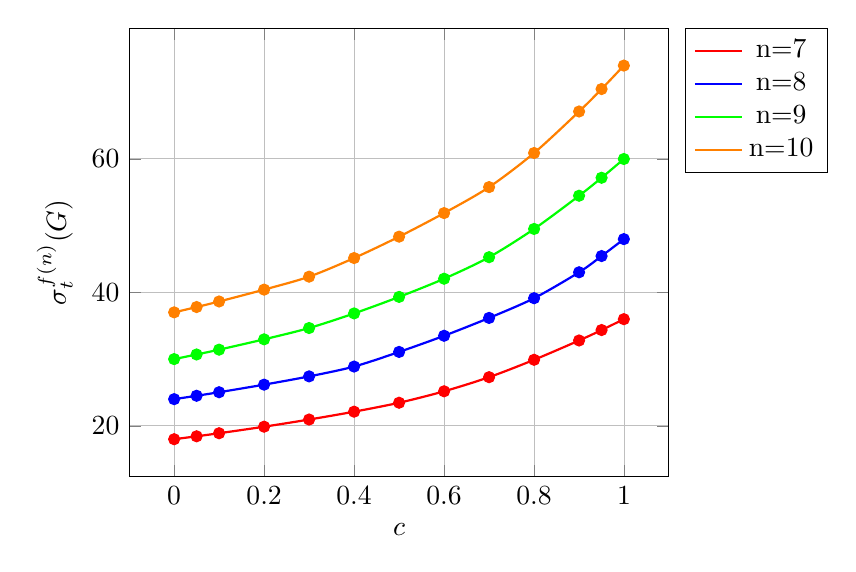
\begin{tikzpicture}
    \begin{axis}[
        xlabel={$c$},
        ylabel={$\sigma_t^{f(n)}(G)$},
        grid=major,
        enlargelimits=true,
        mark size=2pt,
        legend pos=outer north east
    ]
    
    % Interpolacijska črta - 7 vozlišč (rdeča)
    \addplot[
        smooth,
        thick,
        color=red
    ] coordinates {
        (0.0001, 18.001)
        (0.05, 18.437)
        (0.1, 18.895)
        (0.2, 19.875)
        (0.3, 20.948)
        (0.4, 22.124)
        (0.5, 23.463)
        (0.6, 25.178)
        (0.7, 27.293)
        (0.8, 29.897)
        (0.9, 32.789)
        (0.95, 34.352)
        (0.9995, 35.983)
    };

    % Diskretne točke - 7 vozlišč (rdeča)
    \addplot[
        only marks,
        mark=*,
        color=red
    ] coordinates {
        (0.0001, 18.001)
        (0.05, 18.437)
        (0.1, 18.895)
        (0.2, 19.875)
        (0.3, 20.948)
        (0.4, 22.124)
        (0.5, 23.463)
        (0.6, 25.178)
        (0.7, 27.293)
        (0.8, 29.897)
        (0.9, 32.789)
        (0.95, 34.352)
        (0.9995, 35.983)
    };

    % Interpolacijska črta - 8 vozlišč (modra)
    \addplot[
        smooth,
        thick,
        color=blue
    ] coordinates {
        (0.0001, 24.001)
        (0.05, 24.508)
        (0.1, 25.039)
        (0.2, 26.173)
        (0.3, 27.411)
        (0.4, 28.884)
        (0.5, 31.074)
        (0.6, 33.493)
        (0.7, 36.166)
        (0.8, 39.121)
        (0.9, 43.006)
        (0.95, 45.434)
        (0.9995, 47.974)
    };

    % Diskretne točke - 8 vozlišč (modra)
    \addplot[
        only marks,
        mark=*,
        color=blue
    ] coordinates {
        (0.0001, 24.001)
        (0.05, 24.508)
        (0.1, 25.039)
        (0.2, 26.173)
        (0.3, 27.411)
        (0.4, 28.884)
        (0.5, 31.074)
        (0.6, 33.493)
        (0.7, 36.166)
        (0.8, 39.121)
        (0.9, 43.006)
        (0.95, 45.434)
        (0.9995, 47.974)
    };

    % Interpolacijska črta - 9 vozlišč (zelena)
    \addplot[
        smooth,
        thick,
        color=green
    ] coordinates {
        (0.0001, 30.001)
        (0.05, 30.691)
        (0.1, 31.414)
        (0.2, 32.961)
        (0.3, 34.654)
        (0.4, 36.842)
        (0.5, 39.316)
        (0.6, 42.04)
        (0.7, 45.264)
        (0.8, 49.496)
        (0.9, 54.47)
        (0.95, 57.162)
        (0.9995, 59.971)
    };

    % Diskretne točke - 9 vozlišč (zelena)
    \addplot[
        only marks,
        mark=*,
        color=green
    ] coordinates {
        (0.0001, 30.001)
        (0.05, 30.691)
        (0.1, 31.414)
        (0.2, 32.961)
        (0.3, 34.654)
        (0.4, 36.842)
        (0.5, 39.316)
        (0.6, 42.04)
        (0.7, 45.264)
        (0.8, 49.496)
        (0.9, 54.47)
        (0.95, 57.162)
        (0.9995, 59.971)
    };

    % Interpolacijska črta - 10 vozlišč (oranžna)
    \addplot[
        smooth,
        thick,
        color=orange
    ] coordinates {
        (0.0001, 37.002)
        (0.05, 37.797)
        (0.1, 38.63)
        (0.2, 40.407)
        (0.3, 42.347)
        (0.4, 45.137)
        (0.5, 48.341)
        (0.6, 51.871)
        (0.7, 55.762)
        (0.8, 60.87)
        (0.9, 67.088)
        (0.95, 70.452)
        (0.9995, 73.964)
    };

    % Diskretne točke - 10 vozlišč (oranžna)
    \addplot[
        only marks,
        mark=*,
        color=orange
    ] coordinates {
        (0.0001, 37.002)
        (0.05, 37.797)
        (0.1, 38.63)
        (0.2, 40.407)
        (0.3, 42.347)
        (0.4, 45.137)
        (0.5, 48.341)
        (0.6, 51.871)
        (0.7, 55.762)
        (0.8, 60.87)
        (0.9, 67.088)
        (0.95, 70.452)
        (0.9995, 73.964)
    };

    \legend{n=7, , 
            n=8, , 
            n=9, ,
            n=10, }

    \end{axis}
\end{tikzpicture}

\subsection*{Rezultati in ugotovitve}
Ugotovila sva, da so največje vrednosti $\sigma_t^{f(n)}(G)$ za $f(n) = \frac{1}{n}$ dosežene 
pri grafih, ki imajo stopenjsko zaporedje enako kot v izreku. Enako velja za $f(n) = c$,
kjer so vrednosti za $c$ blizu $0$. Nato se na neki točki začneta notranja člena stopenjskega zaporedja zmanjševati, zunanja pa povečevati.
Za $c$ blizu $1$ pa so vrednosti $\sigma_t^{f(n)}(G)$
maksimizirane takrat, ko sta zunanja člena stopenjskega zaporedja $(1^{a_1}, 2^{a_2}, 3^{a_3}, 4^{a_4})$
čim večja, notranja pa čim manjša. Najini algoritmi teh vrednosti niso dosegli, saj sva 
uporabila omejeno število iteracij. Misliva, da za grafe drži naslednja trditev.

Domneva 1 torej drži, domneva 2 pa ne drži, za c blizu 1.

\subsubsection*{Trditev}
Naj bo $n \geq 7$, $f(n) = c$, za $c$ 'zelo blizu' $1$ in naj bo $(1^{a_1}, 2^{a_2}, 3^{a_3}, 4^{a_4})$
stopenjsko zaporedje kemijskega grafa $G$ z maksimalno vrednostjo $\sigma_t^{f(n)}(G)$. Potem velja:
\begin{enumerate}
    \item Če $n = 4k$, potem $a_1 = a_4 = 2k$ in $a_2 = a_3 = 0$.
    \item Če $n = 4k + 1$, potem $a_1 = a_4 = 2k$ in $a_2 = 1$ ($a_3 = 0$) ali $a_3 = 1$ ($a_2 = 0$).
    \item Če $n = 4k + 2$, potem $a_1 = 2k$, $a_2 = 1$, $a_3 = 0$ in $a_4 = 2k + 1$.
    \item Če $n = 4k + 3$, potem $a_1 = 2k - 1$, $a_2 = 0$, $a_3 = 1$ in $a_4 = 2k - 1$.
\end{enumerate}

\subsubsection*{Konstruiranje takih grafov}
Na naslednji strani, sva narisala grafe, ki imajo maksimalno vrednost $\sigma_t^{f(n)}(G)$ za $f(n) = c$,
kjer je c zelo blizu 1. Grafi so narisani za $n \in [16, 19]$ in so le ena od možnosti, zraven
pa sva dodala še njihovo konfiguracijo. Z rdečo so označena vozlišča stopnje 1, z roza 
vozlišča stopnje 2, z zeleno vozlišča stopnje 3 in z modro vozlišča stopnje 4. \\

V splošnem lahko take grafe konstruiramo za poljubno velik $n$. Če je $n = 4k$, potem 
graf konstruiramo tako, da konstruiramo cikel dolžine $2k$, kjer gre ven iz vsakega vozlišča
še ena povezava oziroma list. Na koncu vsako vozlišče, ki je del cikla povežemo z nasprotnje ležečim
vozliščem. \\

Če je $n = 4k + 1$, konstruiramo cikel dolžine $2k$, kjer gre ven iz
vsakega vozlišča še ena povezava. Izberemo poljubnen list, ki mu dodamo še eno povezavo, da 
dobimo graf, ki maksimizira $\sigma_t^{f(n)}(G)$. \\

Če je $n = 4k + 2$, potem konstruiramo cikel dolžine $2k$. Nasprotno ležeča vozlišča povežemo ter
izberemo dve sosednji vozlišči, katerima dodamo novega skupnega soseda. Ostalim tako kot prej dodamo
lsite. Iz soseda prej izbranih dveh vozlišč dodamo še dva lista. Iz enega od novo dodanih listov
dodamo še eno povezavo.  \\

Če je $n = 4k + 3$, konstruiramo cikel dolžine $2k$. Izberemo sosednji vozlišči, ki vsaki dodamo svoj list
ter ta lista povežemo med seboj. Nato enemu od listov dodamo še eno povezavo, drugemu pa dve. Na koncu 
še vsakemu od preostalih vozlišč iz cikla dodamo list. \\




\begin{figure}[H]
    \centering
    % Prva vrstica
    \begin{minipage}{0.48\textwidth}
        \centering
        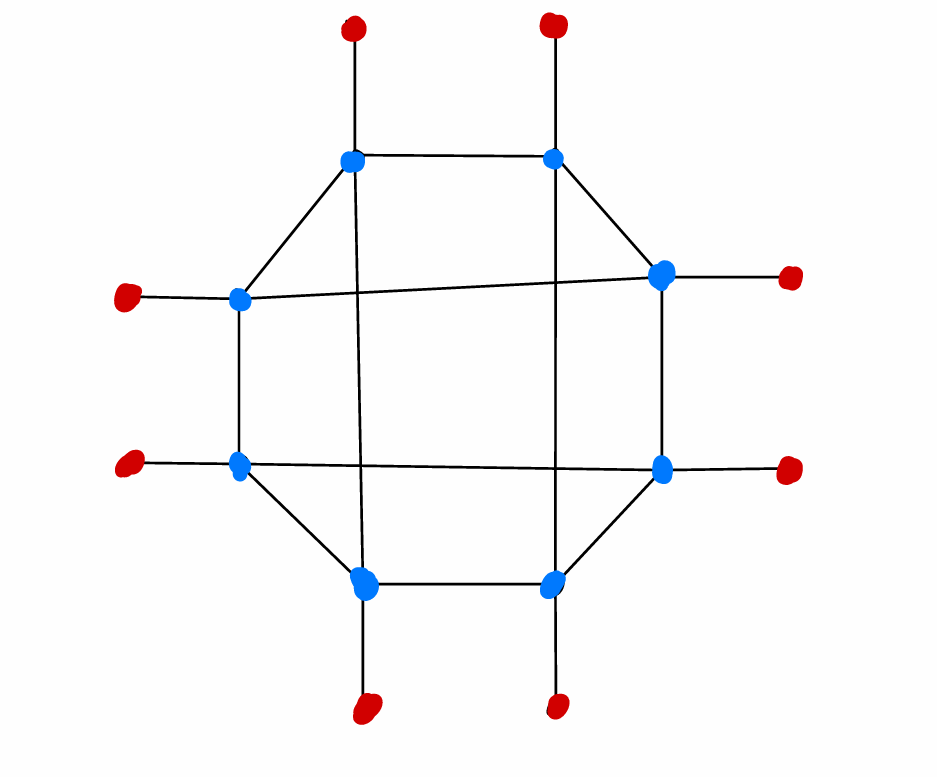
\includegraphics[width=\textwidth]{grafza16.png}
        \caption*{Graf za n = 16; (8, 0, 0, 8)}
    \end{minipage}
    \hfill
    \begin{minipage}{0.48\textwidth}
        \centering
        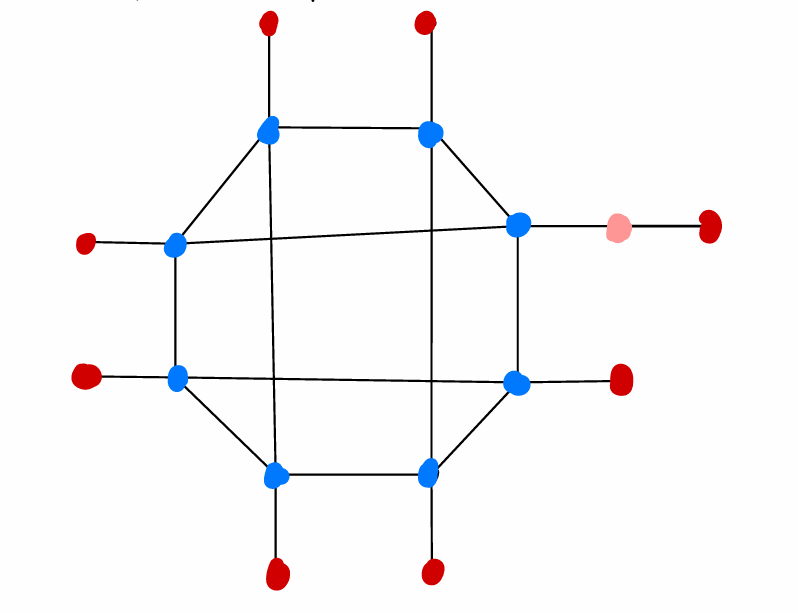
\includegraphics[width=\textwidth]{grafza17.png}
        \caption*{Graf Za n = 17; (8, 1, 0, 8)}
    \end{minipage}

    \vspace{0.5cm} % Razmik med vrsticami

    % Druga vrstica
    \begin{minipage}{0.48\textwidth}
        \centering
        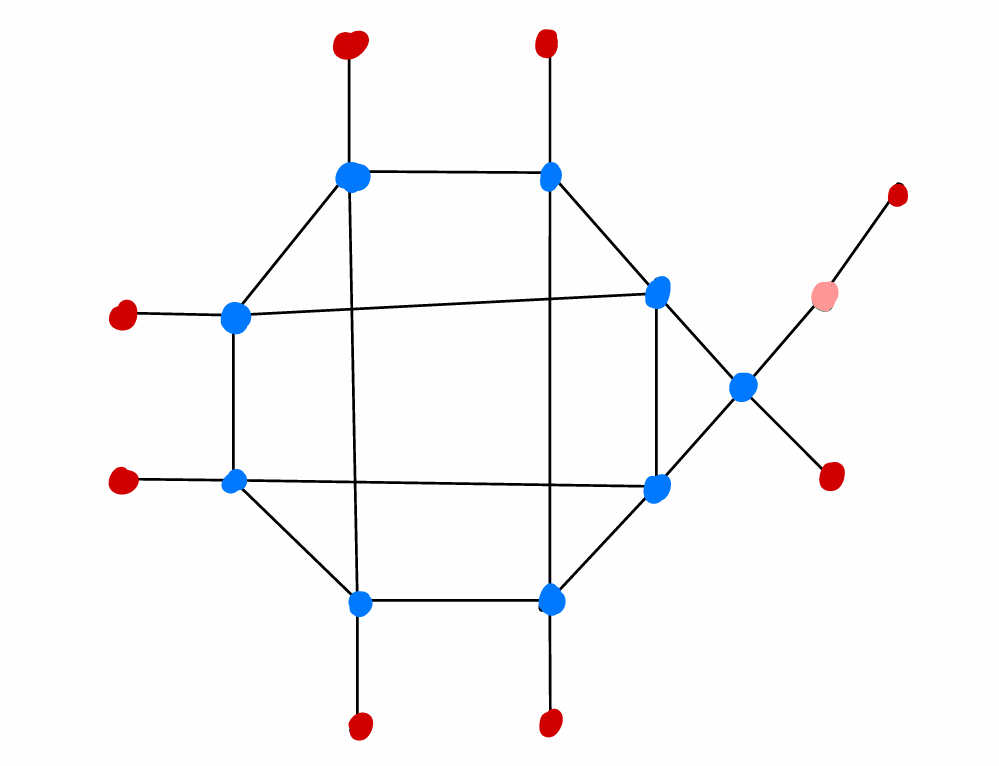
\includegraphics[width=\textwidth]{grafza18.png}
        \caption*{Graf za n = 18; (8, 1, 0, 9)}
    \end{minipage}
    \hfill
    \begin{minipage}{0.48\textwidth}
        \centering
        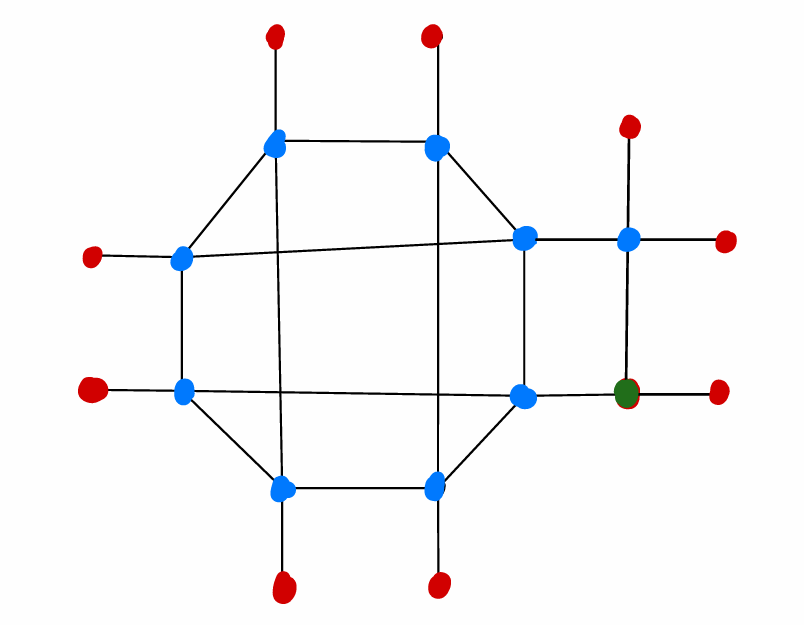
\includegraphics[width=\textwidth]{grafza19.png}
        \caption*{Graf za n = 19; (9, 0, 1, 9)}
    \end{minipage}
    
\end{figure}


\end{document}
